\section{Auswertung}
\label{sec:Auswertung}

%Siehe \autoref{fig:plot}!
\subsection{Berechnung der Landé-Faktoren}
\label{ssec:lande}

Für beide Resonanzstellen werden jeweils die Stromstärken für die Sweep-Spule $I_\text{s}$ und für die Horizontalspule $I_\text{h}$ in Abhängigkeit von der Frequenz $f$.
Mit dem Radius $R$ und der Windungszahl $N$ einer Spule kann über REF ZU HELMHOLTZ das Magentfeld $B$ aus den Stromstärken berechnet werden.
Die Abmessungen der drei Spulen sind 
\begin{align*}
    R_\text{sw} &= \qty{163.90}{\milli\meter} & N_\text{sw} &= \qty{11}{}\\
    R_\text{hor} &= \qty{157.90}{\milli\meter} & N_\text{hor} &= \qty{154}{}\\
    R_\text{ver} &= \qty{117.35}{\milli\meter} & N_\text{ver} &= \qty{20}{}.
\end{align*}
In horizontaler Richtung werden die erzeugten Magnetfelder der Sweep-Spule und der horizontalen Spule addiert.
Die so berechnten Messwerte sind in \autoref{tab:f} notiert.
\begin{table}
    \centering
    \caption{Horizontale Magnetfelder an den Resonanzstellen von beiden Isotopen mit eingestellten Stromstärken der Spulen.}
    \label{tab:f}
    \begin{tabular}{r r r r r r r}
        \toprule
        $f \,/\, \unit{\kilo\hertz}$ & $I_\text{1,s} \,/\, \unit{\ampere}$ & $I_\text{1,h} \,/\, \unit{\ampere}$ & $B_\text{1} \,/\, \unit{\milli\tesla}$ & $I_\text{2,s} \,/\, \unit{\ampere}$ & $I_\text{2,h} \,/\, \unit{\ampere}$ & $B_\text{2} \,/\, \unit{\micro\tesla}$\\
        \midrule
        $100 $ & $625.0\pm1.0$ & $734.0\pm1.0$ & $0.0\pm3.0$ & $0.0\pm3.0$  & $37.7\pm2.6$ & $44.3\pm2.6$ \\
        $200 $ & $440.0\pm1.0$ & $677.0\pm1.0$ & $30.0\pm3.0$ & $30.0\pm3.0$  & $52.9\pm2.6$ & $67.2\pm2.6$ \\
        $300 $ & $422.0\pm1.0$ & $775.0\pm1.0$ & $48.0\pm3.0$ & $48.0\pm3.0$  & $67.6\pm2.6$ & $88.9\pm2.6$ \\
        $400 $ & $296.0\pm1.0$ & $770.0\pm1.0$ & $72.0\pm3.0$  & $72.0\pm3.0 $ & $81.0\pm2.6$ & $109.6\pm2.6$ \\
        $500 $ & $306.0\pm1.0$ & $898.0\pm1.0$ & $90.0\pm3.0$  & $90.0\pm3.0 $ & $97.4\pm2.6$ & $133.1\pm2.6$ \\
        $600 $ & $322.0\pm1.0$ & $710.0\pm1.0$ & $102.0\pm3.0$ & $126.0\pm3.0$ & $108.9\pm2.6$ & $153.3\pm2.6$ \\
        $700 $ & $334.0\pm1.0$ & $698.0\pm1.0$ & $120.0\pm3.0$ & $150.0\pm3.0$ & $125.4\pm2.6$ & $173.7\pm2.6$ \\
        $800 $ & $380.0\pm1.0$ & $432.0\pm1.0$ & $132.0\pm3.0$ & $192.0\pm3.0$ & $138.7\pm2.6$ & $194.4\pm2.6$ \\
        $900 $ & $607.0\pm1.0$ & $554.0\pm1.0$ & $132.0\pm3.0$ & $210.0\pm3.0$ & $152.4\pm2.6$ & $217.6\pm2.6$ \\
        $1000$ & $783.0\pm1.0$ & $710.0\pm1.0$ & $144.0\pm3.0$ & $222.0\pm3.0$ & $173.5\pm2.6$ & $237.5\pm2.6$ \\
        \bottomrule
    \end{tabular}
\end{table}
Die Beziehung zwischen dem Magnetfeld und der Frequenz ist linear, daher eine Gerade durch die Messwerte gelegt.
Dieser wird mit der Python Bibliothen Scipy durchgeführt. QUELLE
Als Fit-Funktion wird dabei eine Gerade der Form
\begin{equation*}
    B(f) = a \cdot f + b
\end{equation*}
genutzt.
Das Ergenis dieses Fits ist in \autoref{fig:frequenz} dargestellt.
\begin{figure}
    \centering
    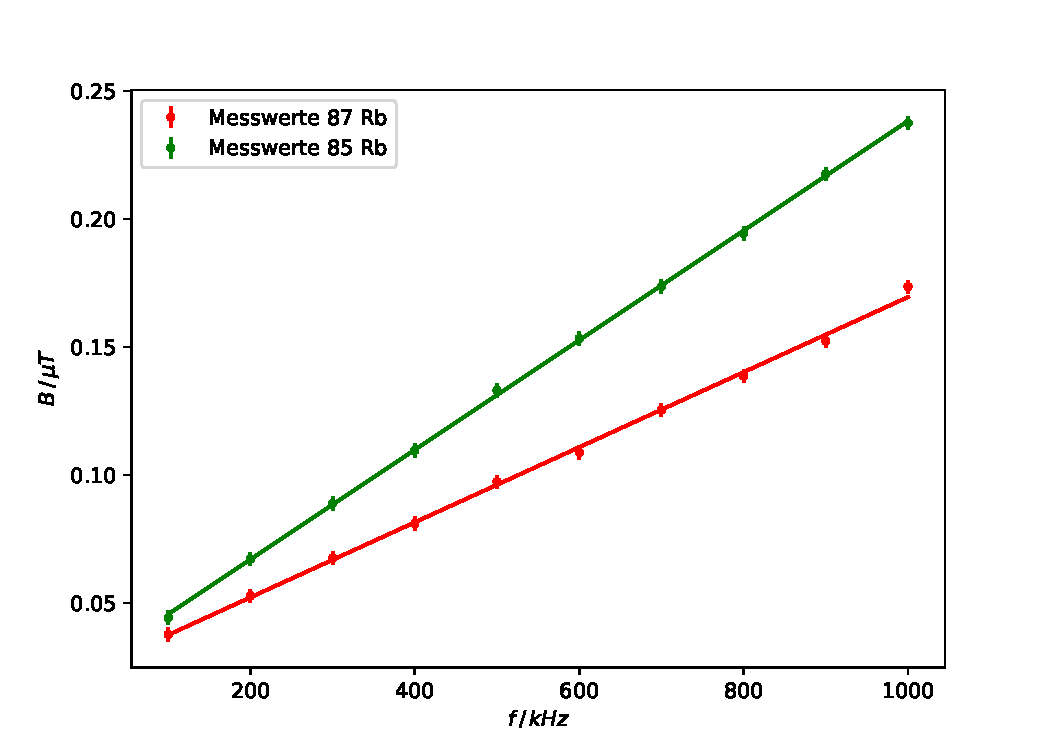
\includegraphics[width=0.8\textwidth]{plots/frequenz.pdf}
    \caption{Fit der Magnetfelder in Abhängigkeit der Frequenz zur Bestimmung der Landé-Faktoren.}
    \label{fig:frequenz}
\end{figure}
Die vom Fit bestimmten Parameter sind 
\begin{align*}
    a_\text{87} &= \qty{1.466(22)e-10}{\per\hertz} \\
    b_\text{87} &= \qty{2.29(13)e-05}{\tesla} \\
    a_\text{85} &= \qty{2.141(29)e-10}{\per\hertz} \\
    b_\text{85} &= \qty{2.42(18)e-05}{\tesla}.
\end{align*}
Wird REF ZUR ZEEMAN GLEICHUNG entsprechend umgestellt, ergibt sich der Zusammenhang
\begin{equation}
    g_\text{f} = \frac{m_\text{e}}{e \cdot a} \cdot 4\pi.
\end{equation}
Darüber wird der Landé-Faktor für beide Isotope 
\begin{align*}
    g_\text{f,87} &= \qty{0.487(7)}{} \\
    g_\text{f,85} &= \qty{0.334(5)}{}.
\end{align*}
bestimmt.

Aus dem Parameter $b$ kann das horizontale Erdmagnetfeld berechnet werden.
Dafür wird der Mittelwert bestimmt.
Damit erhält man für das Erdmagnetfeld
\begin{equation*}
    B_\text{erd} = \qty{2.36(11)e-05}{\tesla}.
\end{equation*}

Zusätzlich kann mit den Landé-Faktoren der Kernspin der Isotopen berechnet werden.
Dafür wird REF ZU FORMEL nach dem Kernspin $I$ umgeformt.
Damit ergeben sich die Kernspins 
\begin{align*}
    I_\text{87} &= \qty{1.552(30)}{} \\
    I_\text{85} &= \qty{2.50(4)}{}.
\end{align*}

\subsection{Isotopenverhältnis}
\label{ssec:verhältnis}

Das Verhältnis der Isotope $\ce{^{87}Rb}$ und $\ce{^{85}Rb}$ kann aus der Tiefe der Resonanzstellen bestimmten werden.
Dafür wird das Oszillatorbild in \autoref{fig:signalbild} verwendet.
Denn das Verhältnis der Minima ist ebenso das Verhältnis der Isotope im Gasgemisch.
\begin{figure}
    \centering
    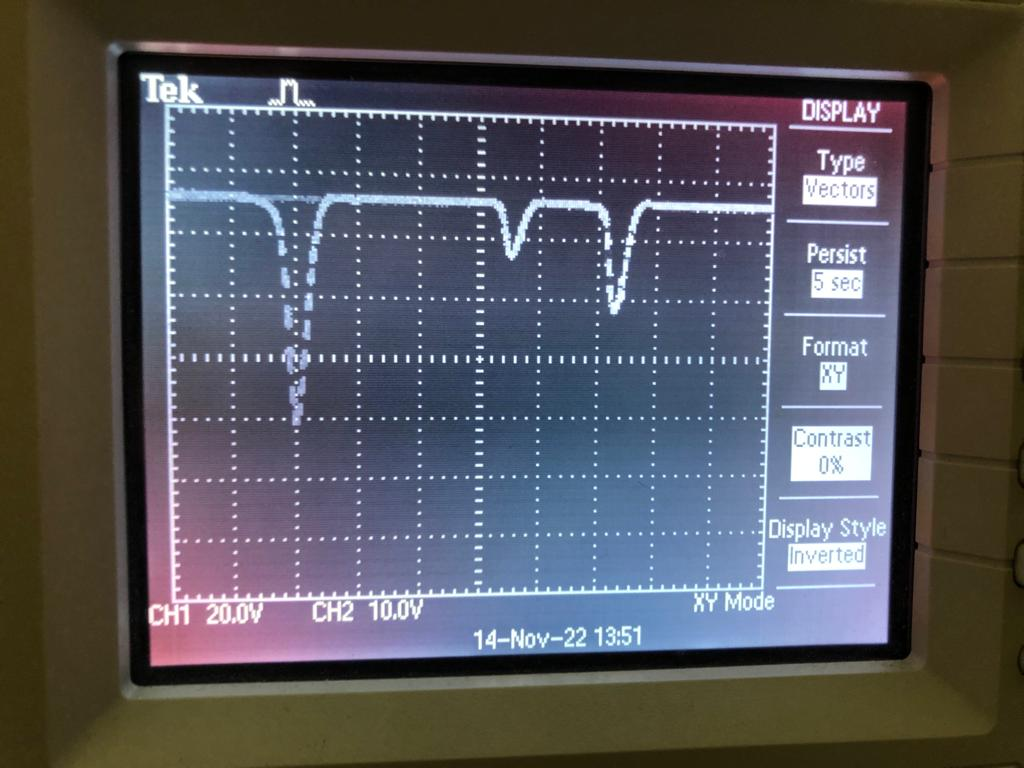
\includegraphics[width=0.8\textwidth]{plots/signalbild.jpeg}
    \caption{Oszillatorbild bei $\qty{100}{\kilo\hertz}$.}
    \label{fig:signalbild}
\end{figure}
Aus dem Bild ergibt sich das Isotopenverhältnis
\begin{equation}
    \frac{0.9 \pm 0.1}{1.7 \pm 0.1} = 0.53 \pm 0.07.
\end{equation}
Daraus wird zusätzlich der prozentuale Anteil für beide Isotope
\begin{align*}
    p_\text{87} &= \qty{34.6(28)}{\percent} \\
    p_\text{85} &= \qty{65.4(28)}{\percent}
\end{align*}
bestimmt.

\subsection{Quadratischer Zeeman-Effekt}
\label{ssec:zeeman}

Bei zu hohen Magnetfeldern treten bei der Zeeman-Aufspaltung quadratische Terme auf.
Über FORMEL kann diese Aufspaltung berechnet werden.
Mit den berechneten Landé-Faktoren $g_\text{f}$, den magnetischen Quantenzahlen $M$ und der Hyperfeinstruktur 
\begin{align*}
    h_{87} &= \qty{4.53e-24}{\joule} 
    h_{85} &= \qty{2.01e-24}{\joule}
\end{align*}
der Isotope kann die quadratische Zeeman-Aufspaltung 
\begin{align*}
    \Delta Z_{87} &= \qty{-4.29(13)e-31}{\joule} 
    \Delta Z_{85} &= \qty{-1.341(29)e-30}{\joule}
\end{align*}
bestimmt werden.

\subsection{Transienten Effekt}
\label{ssec:transient}

Die eingestellten Amplituden der Frequenz und die daraus resultierenden Periodendauern sind in \autoref{tab:A} notiert.
Alle Messwerte sind bei der Resonazstelle von $\qty{100}{\kilo\hertz}$ aufgenommen worden.
\begin{table}
    \centering
    \caption{Periodendauer der Rabi-Oszillationen in Abhängigkeit der RF-Amplitude für beide Isotope.}
    \label{tab:A}
    \begin{tabular}{r r r}
        \toprule
        $A \,/\, \unit{\volt}$ & $T_\text{87} \,/\, \unit{\milli\second}$ & $T_\text{85} \,/\, \unit{\milli\second}$\\
        \midrule
        $1.0 $ & $4.70 $ & $6.00 $\\
        $1.5 $ & $3.16 $ & $4.40 $\\
        $2.0 $ & $2.40 $ & $3.40 $\\
        $2.5 $ & $1.92 $ & $2.80 $\\
        $3.0 $ & $1.68 $ & $2.40 $\\
        $3.5 $ & $1.44 $ & $2.00 $\\
        $4.0 $ & $1.26 $ & $1.90 $\\
        $4.5 $ & $1.12 $ & $1.50 $\\
        $5.0 $ & $0.99 $ & $1.48 $\\
        $6.0 $ & $0.84 $ & $1.20 $\\
        $8.0 $ & $0.60 $ & $0.88 $\\
        $10.0$ & $ 0.47$ & $0.72 $\\
        \bottomrule
    \end{tabular}
\end{table}
Durch die Messwert wird eine hyperpolische Funktion der Form
\begin{equation*}
    T = a + \frac{b}{x - c}
\end{equation*}
gelegt. 
Der Fit wird erneut mit Scipy durchgeführt.
Das Ergbnis ist in \autoref{fig:amplitude} dargestellt.
\begin{figure}
    \centering
    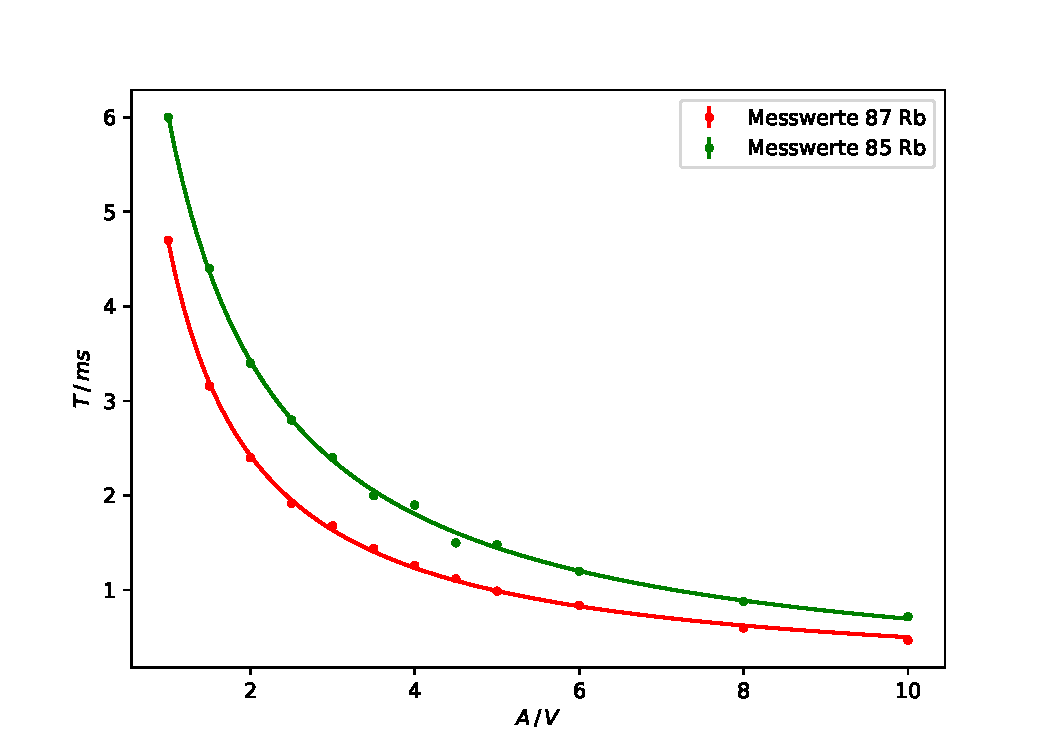
\includegraphics[width=0.8\textwidth]{plots/amplitude.pdf}
    \caption{Hyperbolische Fits der Periodendauern in Abhängigkeit der Frequenzamplitude.}
    \label{fig:amplitude}
\end{figure}
Die daraus resultierenden Parameter sind
\begin{align*}
    a_\text{87} &= \qty{0.7(30)e-05}{\second} & b_{87} &= \qty{0.00499(16)}{\volt\second} &  c_{87} &= \qty{-0.068(31)}{\volt}\\
    a_\text{85} &= \qty{-0.00011(6)}{\second} & b_{85} &= \qty{0.0083(4)}{\volt\second} &  c_{85} &= \qty{-0.36(6)}{\volt}.
\end{align*}
Der Quotient der Parameter $b_{87}$ und $b_{85}$ gibt das Verhältnis der entsprechenden Landé-Faktoren an.
Das Verhältnis ist hier
\begin{equation*}
    \frac{b_{87}}{b_{85}} = \qty{1.67(9)}{}.
\end{equation*}

Um die aufsteigende Flanke ebenfalls mit einer Funktion zu fitten, werden die Messwerte direkt aus den Oszillatorbildern entnommen.
Die Bilder sind in \autoref{fig:oszi} abgebildet.
\begin{figure}
    \centering
    \begin{subfigure}{0.4\textwidth}
        \centering
        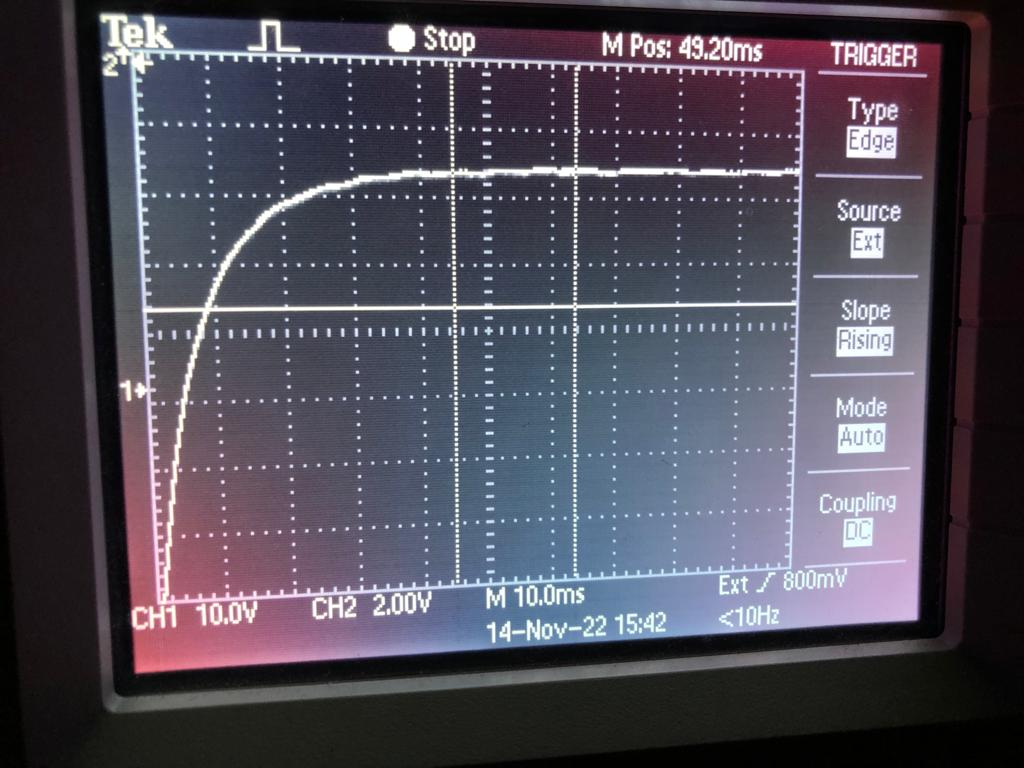
\includegraphics[width=\textwidth]{plots/peak1_5V.jpeg}
        \caption{Oszillatorbild von $\ce{^{87}Rb}$ bei $\qty{5}{\volt}$}
        \label{fig:durchschallung}
    \end{subfigure}
    \begin{subfigure}{0.4\textwidth}
        \centering
        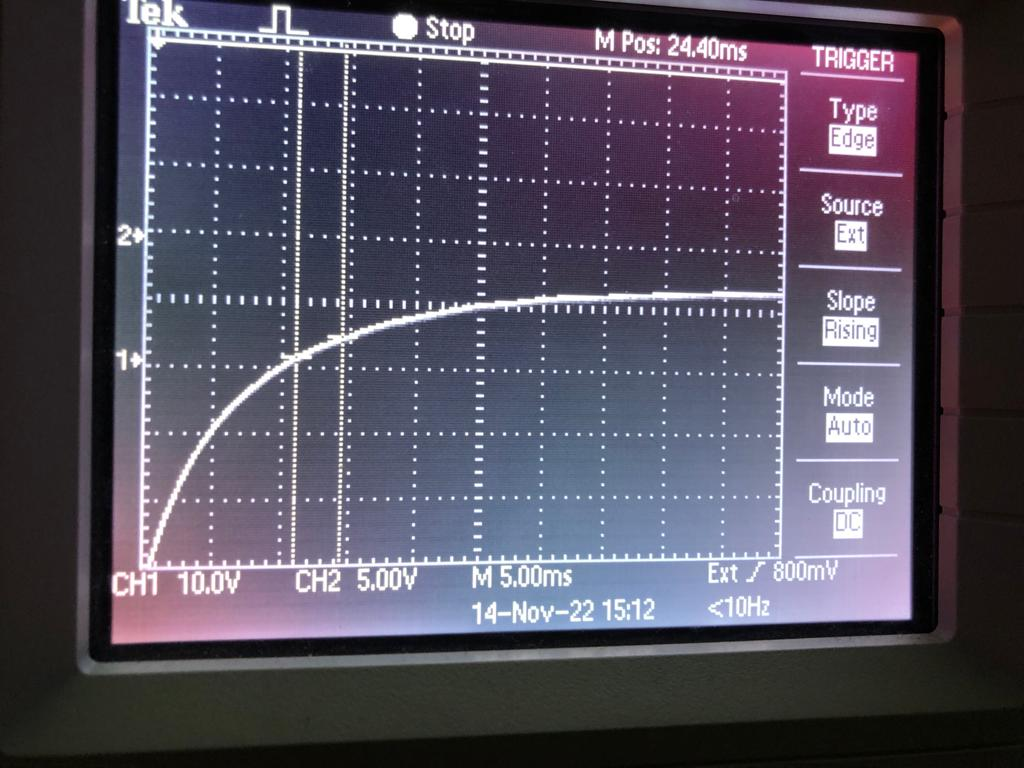
\includegraphics[width=\textwidth]{plots/peak2_2V.jpeg}
        \caption{Oszillatorbild von $\ce{^{85}Rb}$ bei $\qty{2}{\volt}$}
        \label{fig:impuls-echo}
    \end{subfigure}
    \caption{Oszillatorbilder der aufsteigenden Flanke.}
    \label{fig:oszi}
\end{figure}
Daraus werden per Augenmaß die Werte in \autoref{tab:oszi} abgelesen.
\begin{table}
    \centering
    \caption{Periodendauer und detektierte Spannung aus den Oszillatorbildern.}
    \label{tab:oszi}
    \begin{tabular}{r r r r}
        \toprule
        $t_1 \,/\, \unit{\milli\second}$ & $U_\text{87} \,/\, 2 $\cdot$ \unit{\volt}$ & $t_2 \,/\, \unit{\milli\second}$  & $U_\text{85} \,/\, 5 \cdot \unit{\volt}$\\
        \midrule
        $0$   & $0.0\pm 0.1$ & $0$   & $0.0\pm 0.1$\\
        $10$  & $4.6\pm 0.1$ & $5$   & $2.1\pm 0.1$\\
        $20$  & $5.9\pm 0.1$ & $10$  & $3.0\pm 0.1$\\
        $30$  & $6.2\pm 0.1$ & $15$  & $3.5\pm 0.1$\\
        $40$  & $6.3\pm 0.1$ & $20$  & $3.8\pm 0.1$\\
        $50$  & $6.4\pm 0.1$ & $25$  & $4.0\pm 0.1$\\
        $60$  & $6.4\pm 0.1$ & $30$  & $4.1\pm 0.1$\\
        $70$  & $6.4\pm 0.1$ & $35$  & $4.1\pm 0.1$\\
        $80$  & $6.4\pm 0.1$ & $40$  & $4.1\pm 0.1$\\
        $90$  & $6.4\pm 0.1$ & $45$  & $4.1\pm 0.1$\\
        $100$ & $6.4\pm 0.1$ & $50$  & $4.1\pm 0.1$\\
        \bottomrule
    \end{tabular}
\end{table}
Der Fit wird mit einer Exponentialfunktion der Form
\begin{equation*}
    U = a + b \cdot \exp(c \cdot t)
\end{equation*}
durchgeführt und das Ergebnis des Fits sind die Parameter 
\begin{align*}
    a_\text{87} &= \qty{3.195(18)}{} & b_{87} &= \qty{-3.19(5)}{} &  c_{87} &= \qty{-0.127(5)}{}\\
    a_\text{85} &= \qty{0.824(9)}{} & b_{85} &= \qty{-0.819(20)}{} &  c_{85} &= \qty{-0.133(8)}{}.
\end{align*}